\documentclass[10pt,conference]{IEEEtran}
\usepackage{cite}
\usepackage{amsmath,amssymb}
\usepackage{booktabs}
\usepackage{graphicx}
\usepackage{url}
\begin{document}
\title{Interpreting Absent OpenSpec Paths: A Human Decision Tree and a Probability Sample of SpecMine}
\author{\IEEEauthorblockN{Anonymous Authors}}
\maketitle

\begin{abstract}
The SpecMine corpus marks 51,979 OpenSpec task-to-code paths as absent at their reference commits, but a missing path need not signal a defect. We define an ordered eight-class decision tree, reconcile a 90-case human Gold from two reviewers, and use a repository-investigating LLM judge to classify a probability sample of 382 references. With its decision rule fixed before response evaluation, the judge agreed with the frozen Gold on 86/90 cases. Weighted \emph{model-assigned} shares are 34.3\% expected creation, 18.8\% non-file reference, 18.6\% expected move or deletion, 8.4\% external repository, 3.4\% problematic absence, and 13.1\% inaccessible or invalid. Creation labels are more common in open than completed tasks. Sampling intervals exclude model-label error. We release the Gold, probability-sample Silver, decision rules, and case-level provenance. Absence alone does not establish a defect.
\end{abstract}
\begin{IEEEkeywords}
Spec-driven development, mining software repositories, traceability, human annotation, probability sampling.
\end{IEEEkeywords}

\section{Introduction}
Specifications may name code that has not yet been written. Treating every path absent from a repository snapshot as a broken reference can therefore conflate planned work with missing dependencies, a familiar traceability concern~\cite{gotel1994}. SpecMine's July 2026 release records 435,401 OpenSpec task-to-code references; 51,979 literal paths are marked absent at their anchoring commits~\cite{specmine2027}. The MSR Mining Challenge asks how specifications relate to code. We ask a narrower question: \emph{when a path cited in an OpenSpec task is absent at the reference commit, what does that absence permit one to conclude?}

We contribute a measurement instrument and a probability-sampled labeled dataset. An ordered tree distinguishes planned work from missing assumed dependencies while retaining scope errors and unavailable evidence. Two reviewers reconciled a 90-case Gold; a repository-investigating LLM judged 382 sampled Silver cases with design weights and provenance. We analyze model-assigned interpretations without class quotas or corpus-wide classifier extrapolation. SpecMine supplies extracted references and commit-level existence~\cite{specmine2027}; our semantic layer makes the traceability question~\cite{gotel1994} auditable for OpenSpec tasks.

\section{Study Design}
\subsection{Population and unit}
The unit is one task-to-code reference, rather than a task, file, or repository. The target frame contains the 51,979 SpecMine references whose literal paths were recorded as absent at their reference commits and whose sampling keys were available. It spans 4,444 repositories. Mechanical absence is the entry condition; a reviewer may later find a normalized or resolved file at the same commit. Hence \texttt{confirmed\_exists} is possible within this frame. No claim of subsequent implementation follows from an anchor-commit observation.

\subsection{Ordered decision tree}
The same eight-class tree governs human and model decisions (Fig.~\ref{fig:tree}). It first validates the occurrence and commit evidence, then resolves object type and repository scope, and checks file existence at the anchor. For an absent local file, task intent distinguishes creation, move/removal, and a missing assumed dependency; insufficient evidence yields ambiguity. This precedence prevents a current GitHub page or a creation verb from overriding commit and scope evidence. Boundary examples are in the artifact.

\begin{figure*}[t]
\centering
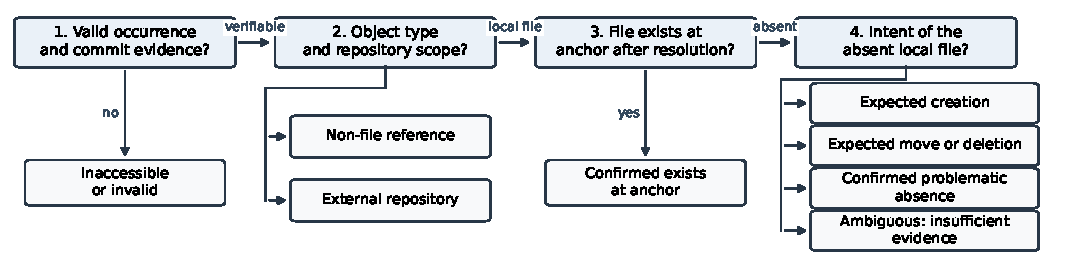
\includegraphics[width=\textwidth]{figures/decision_tree_compact.pdf}
\caption{Ordered decision tree used by both human reviewers and the LLM judge. Follow the upper path only when the preceding gate does not decide the reference. The four outcomes at the last gate depend on task wording and exact-commit repository evidence.}
\label{fig:tree}
\end{figure*}

For example, F001 requests a new test, \path{apps/server/src/db/__tests__/0010_summary_length_check.test.ts}; its absence at the reference commit is expected creation at step 4. F061 instead requests rewriting the existing \path{python/scripts/test_cl_buck.py}, which is absent at its reference commit; step 4 identifies an assumed but missing dependency. Both enter the frame as absent paths, but their task verbs and commit evidence support different interpretations. Source URLs and reviewer notes are in the artifact.

\subsection{Human reference and automated measurement}
The human Gold covers 90 task-to-code references: 30 completed/existing controls, 30 completed/missing, and 30 open/missing, all from different repositories. Reviewer 1 (R1) and Reviewer 2 (R2) initially agreed on 83/90 labels (Cohen's $\kappa=0.8935$)~\cite{cohen1960}; seven disagreements were resolved by consensus. We incorporated these decisions and froze the Gold before comparing the LLM responses. The final set contains three \texttt{confirmed\_missing\_problematic} cases. Its balanced design supports method evaluation, not prevalence estimation.

GPT-6.1 Sol used a fixed tree-aligned prompt, structured eight-class output, read-only exact-commit repository tools, and GitHub search for discovery. The decision rule was finalized before the reported responses were evaluated. The LLM judge could inspect complete task artifacts, other files, paths, and history through the anchor; current web content never replaced commit evidence. Inputs omitted human labels, notes, and the mechanical existence flag. Its traces show 86/90 agreement with the frozen Gold ($\kappa=0.9398$), including 56/60 originally absent cases ($\kappa=0.9033$). Of the three Gold cases labeled \texttt{confirmed\_missing\_problematic}, the LLM judge identified one and classified the other two as expected move or deletion. These were two of the four disagreements overall. Thus, observed sensitivity for the problematic class was 1/3 in this benchmark; with only three such cases, it cannot reliably estimate sensitivity in the population or establish the error rate of the 382 Silver labels.

\subsection{Probability sample and estimation}
A parent random sample of 1,200 absent references was frozen before evidence collection. We selected the first preassigned random ranks within each task-status stratum: 130 open and 252 completed references. This nested 382-case sample covers 296 repositories; no predicted class, access result, or evidence outcome influenced selection. The respective population stratum sizes are 17,752 and 34,227. Each case receives weight $w_h=N_h/n_h$, and the estimated proportion of class $c$ is
\begin{equation}
\hat p_c=\sum_h\frac{N_h}{N}\left(\frac{1}{n_h}\sum_{i\in h}\mathbb{1}[y_i=c]\right).
\end{equation}
We retain inaccessible or invalid records in the denominator. Our estimand is the finite-frame share \emph{assigned} to each class by the judge, not the unknown share of correct human interpretations. The conventional worst-case 95\% margin with finite population correction is approximately 5.0 percentage points for an overall proportion near 0.5 under reference-level sampling. Table~\ref{tab:dist} gives approximate weighted Wilson intervals using the effective sample size; these describe sampling variation in model-assigned shares. Neither the margin nor the intervals includes model-label error or frame error. They are not simultaneous guarantees for all eight classes.

\section{Results}
All 382 cases have one valid classification and a complete case trace. The judge attempted to read the reference-commit artifact for every case: 348 reads found it, 32 reported an unavailable commit, and two did not find the artifact at that commit. It made 1,007 repository-tool calls and five web searches. No prohibited label fields appeared in the starting records. One malformed response was rerun once without changing the frozen configuration. Two sampled references overlap the 90-case Gold benchmark and remain in the probability estimate; excluding them changes each reported share by less than 0.2 percentage points.

\begin{table}[t]
\caption{LLM-assigned classes among 51,979 mechanically absent references. Weighted estimates and approximate 95\% intervals describe sampling variation, not label error.}
\label{tab:dist}
\centering\scriptsize
\begin{tabular}{p{3.35cm}rr}
\toprule
\textbf{Interpretation} & \textbf{Cases} & \textbf{Estimate [95\% interval]}\\
\midrule
Expected creation & 131 & 34.3\% [29.7, 39.2]\\
Expected move or deletion & 71 & 18.6\% [15.0, 22.8]\\
Non-file reference & 72 & 18.8\% [15.2, 23.1]\\
External repository & 32 & 8.4\% [6.0, 11.6]\\
Inaccessible or invalid & 50 & 13.1\% [10.1, 16.8]\\
Confirmed problematic absence & 13 & 3.4\% [2.0, 5.7]\\
Confirmed exists after resolution & 13 & 3.4\% [2.0, 5.7]\\
Ambiguous & 0 & 0.0\% [0.0, 1.0]\\
\bottomrule
\end{tabular}
\end{table}

Expected creation or move/removal accounts for 52.9\% of weighted model assignments (exploratory design-based 95\% interval [47.9, 57.9]); even for model labels, a strict majority is not established. Scope or non-file interpretations account for 27.2\%. Creation exceeds each of the next two classes by about 15.5 percentage points; exploratory design-based difference intervals are [8.5, 22.5] points versus non-file and [8.8, 22.7] versus move/removal. Non-file and move/removal differ by only 0.3 points (interval [-5.9, 6.4]); their ordering is unresolved by sampling. Only 13 cases received a problematic label (3.4\% weighted), and 13.1\% were inaccessible/invalid. The two missed problematic Gold cases make this rare-class share especially uncertain; neither the share nor its sampling interval establishes the true problematic rate. Among the 332 semantically classifiable cases, creation accounts for 39.5\%, a conditional result that excludes unavailable evidence.

The judge assigned creation to 64/130 open cases (49.2\%) and 67/252 completed cases (26.6\%): a 22.6-point open-minus-completed difference (exploratory design-based interval [12.5, 32.8]). It assigned move/removal to 11.5\% and 22.2\%, respectively (difference -10.7 points; interval [-18.2, -3.2]). These unadjusted contrasts concern model labels and sampling variation only; they neither observe transitions nor establish an effect of task status.

\section{Discussion and Implications}
The answer to our question is conditional: absence establishes that a literal path was not found by a particular resolver at a particular commit. It does not by itself identify a defect, a hallucinated file, abandoned work, or successful later implementation. The ordered tree supplies the additional evidence needed to make narrower conclusions. For a repository tool, a missing-path alert should prompt commit-aligned checks of object type, scope, and task intent before claiming a defect. The F001/F061 contrast illustrates why treating every missing path alike would misrepresent both planned work and assumed existing dependencies.

The released Silver is useful for future studies because each sampled reference carries its selection weight, source identifiers, model-assigned class, rationale, and investigative trace. It is an auditable measurement output, not 382 human-confirmed labels. The frozen Gold documents the two-reviewer consensus and pre-comparison methodological corrections. For scale, moving ten weighted-near-equal sample cases into or out of one class would change its estimated share by about 2.6 percentage points; this illustrative perturbation is not an error bound. The broad observation that literal absence has several plausible meanings is supported by the tree and human cases, while the exact class shares depend on the judge's unmeasured error. Future work can audit a fresh probability subset and investigate rare classes or later implementation.

\section{Threats to Validity}
\emph{Measurement:} The 90-case benchmark was deliberately balanced and contains only three problematic Gold cases, limiting conclusions about class-specific performance. Later model-informed human decisions were excluded. No independent human audit of the population sample was conducted, so the 86/90 benchmark agreement does not quantify Silver-label error. The 50 inaccessible/invalid Silver cases may hide a different class mix. Evidence available to the judge may also differ from what humans saw, despite commit anchoring.

\emph{Sampling and inference:} The frame inherits SpecMine's extraction and path-resolution choices. References are the randomly selected units, so the reported intervals target finite-frame reference shares; they do not support repository-level or future-corpus inference. The nested selection preserves the pre-evidence random ranking, but any frame omissions remain outside our estimand. Approximate intervals and exploratory contrasts exclude model error; the contrast intervals are not adjusted for multiple comparisons. Class-specific margins are wider or unstable for rare outcomes. The 90-case Gold was deliberately balanced across task/existence groups and does not estimate prevalence.

\emph{Interpretation:} Task wording and repository evidence support an intent-based classification at one commit. They cannot establish downstream delivery, developer intent beyond recorded artifacts, or causality. Findings apply to OpenSpec references in this SpecMine release; transfer to other specification systems needs study.

\section{Ethical Implications}
The analysis uses public repository material while preserving source attribution and commit provenance. Personal identifiers are not study variables; the review archive replaces incidental email-like strings and user-home path segments with documented placeholders. Automated labels can be wrong, especially for rare classes, so the dataset should support research and review rather than judgments about developer quality.

\section{Conclusion and Data Availability}
In the probability sample, the judge most often classified literally absent OpenSpec paths as planned creation. Non-file and move/removal assignments were similarly frequent, while creation assignments were more frequent for open than completed tasks. The true population distribution, particularly problematic absence, remains sensitive to unmeasured classification error. We contribute an explicit decision procedure, a frozen human Gold, and a probability-sampled model Silver dataset with case-level provenance. An anonymous artifact link will be added after the release package passes double-anonymous checks.

\bibliographystyle{IEEEtran}
\bibliography{references}
\end{document}
